\subsubsection*{PowerStack}

\paragraph{Overview} 
Power remains a critical constraint for Exascale. As we design supercomputers with higher heterogeneity at larger scales, power becomes an expensive and limited resource. Inefficient management of power leads to added operational costs as well as low scientific throughput. Although hardware advances will contribute a certain amount towards achieving high energy efficiency, several vendors agree that these will not be sufficient in isolation -- creating a need for a sophisticated system software approach. Significant advances in software technologies are thus required to ensure that Exascale systems achieve high performance with effective utilization of available power. Distributing available power to nodes (and components such as GPUs) while adhering to system, job and node constraints involves complex decision making in software. 

The ECP PowerStack sub-area in Argo explores hierarchical interfaces for power management at three specific levels: batch job schedulers, job-level runtime systems, and node-level managers. Each level will provide options for adaptive management depending on requirements of the supercomputing site under consideration. Site-specific requirements such as cluster-level power bounds, user fairness, or job priorities will be translated as inputs to the job scheduler. The job scheduler will choose power-aware scheduling plugins to ensure compliance, with the primary responsibility being management of allocations across multiple users and diverse workloads. Such allocations (physical nodes and job-level power bounds) will serve as inputs to a fine-grained, job-level runtime system to manage specific application ranks, in-turn relying on vendor-agnostic node-level measurement and control mechanisms. The figure below presents an overview of the envisioned PowerStack, which takes a holistic approach to power management.  Additionally, power management support for science workflows (such as MuMMI Cancer workflow, E3SM climate models, etc), in-situ visualization, and workflow management infrastructures (e.g. Kokkos and Caliper) is being developed. Interfaces with ATDM projects such as LLNL's Flux are also being developed. Furthermore, solutions for co-scheduling challenges for extremely heterogeneous architectures are being designed as a part of a university subcontract to University of Arizona. 

This project is essential for ECP because it enables power management of Exascale applications and science workflows on modern heterogeneous architectures, where optimal performance often depends on how resources are scheduled efficiently across power domains (eg GPUs, or co-scheduling). The project is also essential to allow for better throughput and utilization of such heterogeneous clusters, and for allowing applications to operate safely and optimally with power and energy constraints when needed. This project is also essential for building a sophisticated hierarchical software stack proposed by the ECP ATDM (LLNL) and Flux projects, as well as community standardization efforts such as the PowerAPI standard. Additionally, the project fulfills an essential need for ECP by enabling vendor and academic collaborations that provide for accelerated adoption of best practices and better interoperability at scale. By leveraging the software developed in this project, compute centers can safely operate under power and energy constraints while maximizing performance and scientific throughput. 

\begin{figure}[t]
	\centering
	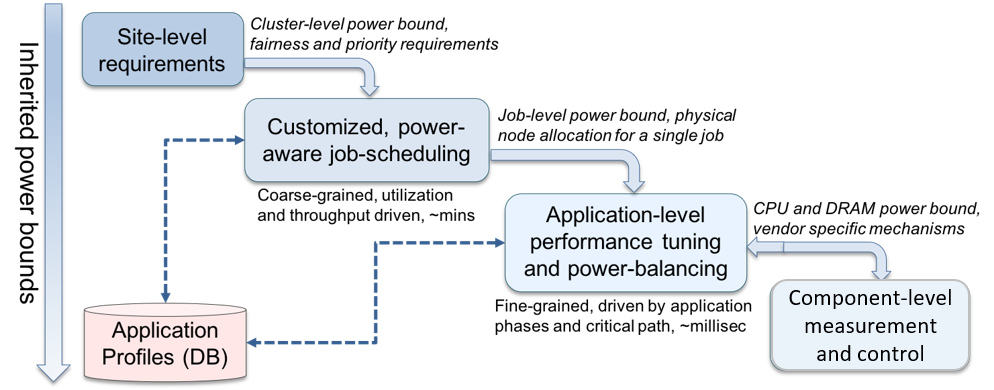
\includegraphics[scale = 0.7]{projects/2.3.1-PMR/2.3.1.19-Argo-PowerSteering/PowerStack_v2.png}
	\caption{Envisioned PowerStack}
	\label{fig:pstack}
\end{figure}


\paragraph{Key Challenges}
Power management in software is challenging due to the dynamic phase behavior of applications, processor manufacturing variability, and the increasing heterogeneity of node-level components. While several scattered research efforts exist, a majority of these efforts are site-specific, require substantial programmer effort, and often result in suboptimal application performance and system throughput. Additionally, these approaches are not production-ready and are not designed to cooperate in an integrated manner. A holistic, generalizable and extensible approach is still missing in the HPC community, and a goal for the ECP Argo PowerSteering project is to provide a solution for this technology gap. 

Another set of challenges come from portability issues. Existing solutions are targeted toward specific microarchitectures (typically Intel) as well as specific programming models (typically MPI-only and traditional benchmarks). Additionally, some of the existing solutions violate the specified power budget before reaching a steady state, resulting in power fluctuations as well as unsafe operation. As part of this project, we strive to provide portability across multiple platforms (IBM, NVIDIA, ARM, AMD, etc), multiple programming models that enable workflows (through Kokkos or Caliper, or specific science workflow studies such as E3SM or MuMMI). Such portability and support of vendor-neutrality is important for safe operation using both hardware-level and application-level information for adaptive configuration selection and critical path analysis.

\paragraph{Solution Strategy}
As discussed earlier, our solution is to develop an end-to-end deployable stack, that combines coarse-grained power-scheduling (Flux, SLURM) with fine-grained job-level runtime system (Intel GEOPM) while ensuring vendor neutrality through node-level interfaces in Variorum. Such a stack can typically operate transparently to user applications. At the scheduler level, we are working on extending SLURM and Flux resource managers to be power-aware. Here, we are looking at both static, coarse-grained power management and variation-aware scheduling in Flux, as well as portability through SLURM SPANK plugins. For the \emph{job-level}, a power management runtime system called GEOPM that will optimize performance of Exascale scientific applications transparently is being developed in collaboration with Intel. At the node-level, vendor-neutral interfaces are being developed as part of Variorum library, to allow for support for Intel, IBM, AMD, ARM, and HPE/Cray platforms. In order to accomplish portability and smooth integration across domains, we are closely collaborating with ECP MuMMI workflow project, the E3SM workflow project, ECP Flux, Kokkos and Caliper, and with the University of Arizona. We are actively engaging ECP users in order to support power management in a non-intrusive and transparent manner. 

\paragraph{Recent Progress}
We achieved three milestones through FY20 in September 2020. The first was to release a production-ready version of Variorum, a vendor neutral power monitoring and control library, with support for Intel, IBM and NVIDIA platforms. Variorum currently supports IBM Witherspoon architecture with Power9, NVIDIA Volta GPUs, and six Intel microarchitectures (Sandy Bridge, Ivy Bridge, Haswell, Broadwell, Kaby Lake, Skylake) in a vendor-neutral manner. Our second milestone this year was the initial deployment and testing of a production-ready PowerStack. Here, we first developed interfaces between Intel GEOPM and Variorum to allow for vendor-neutral access across the platforms that Variorum supports. Then, we tested and included GEOPM v1.1 as a part of the TOSS (Tri-Lab Operating System) release, which included significant testing and integration. This now allows users on the Tri-Lab systems with the underlying platforms (currently Intel) to utilize GEOPM. Additionally, we implemented SLURM SPANK plugins through msr-safe to allow for resource management level control.  We also tested our Flux variation-aware plugin, which was developed last year as part of ECP Argo for the second milestone.  For our third milestone, we carried out power and performance analysis of the MuMMI Cancer Workflow, explored power management of co-scheduled applications by studying NAS benchmarks and E3SM configurations, and delivered a Kokkos-tool extension to Variorum. We began the process of understanding how we can write a Caliper service for Variorum as well. 
In parallel, as part of ASC L2 for the Flux effort, Flux and Variorum integration was also carried out for upcoming supercomputers for both power monitoring and capping (outside of the scope of this ECP Argo PowerSteering project, but expected to help with integration efforts at exascale).
Additionally, LLNL is working on a multi-vendor CRADA involving Intel, HPE, ARM and IBM -- industry partners that are helping us drive vendor-neutral solutions to power management; and are actively engaged in the community effort for PowerStack homogenization. We are also working in collaboration with PowerAPI team for the same. We established the PowerStack community charter in June 2018, involving collaborators across multiple vendors (Intel, IBM, ARM, HPE, AMD, NVIDIA, Cray), academic institutions (TU Munich, Univ. Tokyo, Univ. Bologna, Univ. Arizona), and national laboratories (Argonne National Lab).The goal for this team is to design a holistic, flexible and extensible concept of a software stack ecosystem for power management. Over the past 2.5 years, this group is looking at engineering and research challenges, along with RFP/procurement designs through active vendor interaction and involvement. We held a 3-day seminar in Nov 2019 and again in June 2020 virtually this year, the details of which can be found here: \url{https://hpcpowerstack.github.io/powerstack-nov19.html}. 

\paragraph{Next Steps}
We will continue our research and development work as planned toward the FY21 milestones. More specifically, we will continue development for variorum library to allow support for ARM, AMD and other architectures. We will continue to extend Intel GEOPM's new codebase, continue development of scheduler components such as Flux and SLURM, work on GPU power capping research, and enable user-space access to power management on diverse architectures. We will expand our collaborations for science workflows, such as MuMMI and E2SM, including support for Caliper and Kokkos power management. We will also continue to further explore co-scheduling challenges in power management (University of Arizona) and multi-tenancy issues in power management on heterogenous architectures, and lead the efforts on multi-vendor CRADA. 
